% !TeX root = 系统动力学建模与仿真笔记.tex
广义变分原理在诸多学科中均有广泛应用，维数上包括有限维和无限维两种情形。在多体系统动力学建模中主要涉及有限维形式的广义变分原理，为此本章简述有限维广义变分原理的内容及其证明过程，并以多元函数极值问题的求解为例简要说明原理的应用，为后续多体系统动力学建模奠定理论基础。

\section{独立变分原理}

\begin{myTheorem}{独立变分原理}
对于 $n$ 维实数列阵 $\bm{a} \in \mathbb{R}^n$ 和 $\bm{q} \in \mathbb{R}^n$，若 $\bm{q}$ 的任意微小变更 $\delta\bm{q}$ 与 $\bm{a}$ 的内积均为零，则 $\bm{a}$ 为零列阵。
\end{myTheorem}

\noindent 简记形式：$\bm{a} \in \mathbb{R}^n$，$\bm{q} \in \mathbb{R}^n$，
\begin{equation}\label{eq:1.9}
\delta\bm{q}^{\mathrm{T}} \bm{a} = 0, \quad \forall\, \delta\bm{q} \quad \Rightarrow \quad \bm{a} = \bm{0}.
\end{equation}

\begin{proof}
对于 $\bm{q}$ 的任意微小变更 $\delta\bm{q}$ 都有
\begin{equation}\label{eq:1.10}
\delta\bm{q}^{\mathrm{T}} \bm{a} = 0.
\end{equation}
令
\begin{equation}\label{eq:1.11}
\delta\bm{q} = \begin{bmatrix} 0 & \cdots & 0 & \delta q_k & 0 & \cdots & 0 \end{bmatrix}^{\mathrm{T}}, \quad \delta q_k \neq 0.
\end{equation}
将式~(\ref{eq:1.11})~代入式~(\ref{eq:1.10})~整理可得
\begin{equation}\label{eq:1.12}
0 = \delta\bm{q}^{\mathrm{T}} \bm{a} = \delta q_k \, a_k, \quad \Rightarrow \quad a_k = 0.
\end{equation}
考虑到下标 $k$ 的任意性，由式~(\ref{eq:1.12})
\begin{equation}\label{eq:1.13}
a_k = 0 \quad (k = 1, 2, \cdots, n).
\end{equation}
由此可得
\begin{equation}\label{eq:1.14}
\bm{a} = \bm{0}.
\end{equation}
\end{proof}

\section{非独立变分原理}

\parahead{不含冗余约束的有限维非独立变分}

\begin{myTheorem}{不含冗余约束的有限维非独立变分原理}
对于 $n$ 维实数列阵 $\bm{a} \in \mathbb{R}^n$ 和 $\bm{q} \in \mathbb{R}^n$，以及 $m \times n$ 维行满秩矩阵 $\bm{\Phi} \in \mathbb{R}^{m \times n}$，在满足$m$个约束方程 $\bm{\Phi}\,\delta\bm{q} = \bm{0}$ 的前提下，如果 $\bm{q}$ 的任意微小变更 $\delta\bm{q}$ 与 $\bm{a}$ 的内积均为零，即 $\delta\bm{q}^{\mathrm{T}} \bm{a} = 0$，则存在 $m$ 维拉格朗日乘子 $\bm{\lambda} \in \mathbb{R}^m$ 使得 $\bm{a}$ 与 $\bm{\Phi}^{\mathrm{T}} \bm{\lambda}$ 的和为零。\\

 简记形式：$\bm{a} \in \mathbb{R}^n$，$\bm{q} \in \mathbb{R}^n$，$\bm{\Phi} \in \mathbb{R}^{m \times n}$，$\operatorname{rank}(\bm{\Phi}) = m$，
\begin{equation}\label{eq:1.24}
	\delta\bm{q}^{\mathrm{T}} \bm{a} = 0, \quad \forall\, \delta\bm{q} : \bm{\Phi}\,\delta\bm{q} = \bm{0} \quad \Rightarrow \quad \exists\, \bm{\lambda} \;\text{s.t.}\; \bm{a} + \bm{\Phi}^{\mathrm{T}} \bm{\lambda} = \bm{0}.
\end{equation}
\end{myTheorem}



\begin{proof}
行满秩矩阵 $\bm{\Phi} \in \mathbb{R}^{m \times n}$ 的维数一定满足
\begin{equation}\label{eq:1.25}
m \leq n.
\end{equation}

通过基本的列变换，约束方程系数矩阵 $\bm{\Phi} \in \mathbb{R}^{m \times n}$ 可转换为如下形式
\begin{equation}\label{eq:1.26}
\bm{\Phi} \bm{C} = \begin{bmatrix} \bm{\Phi}_D & \bm{\Phi}_I \end{bmatrix},
\end{equation}
式中 $\bm{C}$ 为可逆的列变换矩阵；$\bm{\Phi}_D \in \mathbb{R}^{m \times m}$ 为可逆矩阵，$\bm{\Phi}_I \in \mathbb{R}^{m \times (n-m)}$。根据式~(\ref{eq:1.26})~对变分约束条件 $\bm{\Phi}\,\delta\bm{q} = \bm{0}$ 作如下等价变换，即
\begin{equation}\label{eq:1.27}
\bm{0} = \bm{\Phi}\,\delta\bm{q} \iff \bm{0} = \bm{\Phi} \bm{C}\, \bm{C}^{-1} \delta\bm{q} = \begin{bmatrix} \bm{\Phi}_D & \bm{\Phi}_I \end{bmatrix} \bm{C}^{-1} \delta\bm{q}.
\end{equation}
若令
\begin{equation}\label{eq:1.28}
\delta\bar{\bm{q}} \triangleq \bm{C}^{-1} \delta\bm{q},
\end{equation}
则有
\begin{equation}\label{eq:1.29}
\delta\bm{q} = \bm{C}\,\delta\bar{\bm{q}},
\end{equation}
此时变分约束条件~(\ref{eq:1.27})~可进一步等效为
\begin{equation}\label{eq:1.30}
\bm{0} = \bm{\Phi}\,\delta\bm{q} \iff \bm{0} = \begin{bmatrix} \bm{\Phi}_D & \bm{\Phi}_I \end{bmatrix} \delta\bar{\bm{q}}.
\end{equation}
进一步，可将 $\delta\bar{\bm{q}}$ 记为如下分块形式，即
\begin{equation}\label{eq:1.31}
\delta\bar{\bm{q}} =: \begin{bmatrix} \delta\bar{\bm{q}}_D \\ \delta\bar{\bm{q}}_I \end{bmatrix},
\end{equation}
式中，$\delta\bar{\bm{q}}_D \in \mathbb{R}^m$，$\delta\bar{\bm{q}}_I \in \mathbb{R}^{n-m}$。此时变分约束条件~(\ref{eq:1.30})~可进一步等效为
\begin{equation}\label{eq:1.32}
\bm{0} = \bm{\Phi}\,\delta\bm{q} \iff \bm{0} = \bm{\Phi}_D \,\delta\bar{\bm{q}}_D + \bm{\Phi}_I \,\delta\bar{\bm{q}}_I.
\end{equation}
考虑到 $\bm{\Phi}_D \in \mathbb{R}^{m \times m}$ 为可逆矩阵，变分约束条件~(\ref{eq:1.32})~可进一步等效为
\begin{equation}\label{eq:1.33}
\bm{0} = \bm{\Phi}\,\delta\bm{q} \iff \delta\bar{\bm{q}}_D = -\bm{\Phi}_D^{-1} \bm{\Phi}_I \,\delta\bar{\bm{q}}_I.
\end{equation}

考虑到式~(\ref{eq:1.29})，内积为零的条件 $0 = \delta\bm{q}^{\mathrm{T}} \bm{a}$ 可等效为
\begin{equation}\label{eq:1.34}
0 = \delta\bm{q}^{\mathrm{T}} \bm{a} \iff 0 = \delta\bar{\bm{q}}^{\mathrm{T}} \bm{C}^{\mathrm{T}} \bm{a}.
\end{equation}
若令
\begin{equation}\label{eq:1.35}
\bar{\bm{a}} \triangleq \bm{C}^{\mathrm{T}} \bm{a},
\end{equation}
则有
\begin{equation}\label{eq:1.36}
\bm{a} = \bm{C}^{-\mathrm{T}} \bar{\bm{a}},
\end{equation}
此时内积为零的条件~(\ref{eq:1.34})~可进一步等效为
\begin{equation}\label{eq:1.37}
0 = \delta\bm{q}^{\mathrm{T}} \bm{a} \iff 0 = \delta\bar{\bm{q}}^{\mathrm{T}} \bar{\bm{a}}.
\end{equation}
进一步，可将 $\bar{\bm{a}}$ 记为如下分块形式，即
\begin{equation}\label{eq:1.38}
\bar{\bm{a}} =: \begin{bmatrix} \bar{\bm{a}}_D \\ \bar{\bm{a}}_I \end{bmatrix},
\end{equation}
式中，$\bar{\bm{a}}_D \in \mathbb{R}^m$，$\bar{\bm{a}}_I \in \mathbb{R}^{n-m}$。此时内积为零的条件~(\ref{eq:1.37})~可进一步等效为
\begin{equation}\label{eq:1.39}
0 = \delta\bm{q}^{\mathrm{T}} \bm{a} \iff 0 = \delta\bar{\bm{q}}_D^{\mathrm{T}} \bar{\bm{a}}_D + \delta\bar{\bm{q}}_I^{\mathrm{T}} \bar{\bm{a}}_I.
\end{equation}

由变分约束条件~(\ref{eq:1.33})~和内积为零的条件~(\ref{eq:1.39})~可知，对于任意的微小变更 $\delta\bar{\bm{q}}_I$，有
\begin{equation}\label{eq:1.40}
\begin{aligned}
0 &= \delta\bar{\bm{q}}_D^{\mathrm{T}} \bar{\bm{a}}_D + \delta\bar{\bm{q}}_I^{\mathrm{T}} \bar{\bm{a}}_I \\
&= -\delta\bar{\bm{q}}_I^{\mathrm{T}} \bm{\Phi}_I^{\mathrm{T}} \bm{\Phi}_D^{-\mathrm{T}} \bar{\bm{a}}_D + \delta\bar{\bm{q}}_I^{\mathrm{T}} \bar{\bm{a}}_I \\
&= \delta\bar{\bm{q}}_I^{\mathrm{T}} \!\left( -\bm{\Phi}_I^{\mathrm{T}} \bm{\Phi}_D^{-\mathrm{T}} \bar{\bm{a}}_D + \bar{\bm{a}}_I \right).
\end{aligned}
\end{equation}
则由独立变分原理~(\ref{eq:1.9})~可得
\begin{equation}\label{eq:1.41}
-\bm{\Phi}_I^{\mathrm{T}} \bm{\Phi}_D^{-\mathrm{T}} \bar{\bm{a}}_D + \bar{\bm{a}}_I = \bm{0}.
\end{equation}

进一步，可将表达式~(\ref{eq:1.41})~中的乘积项 $-\bm{\Phi}_D^{-\mathrm{T}} \bar{\bm{a}}_D$ 记为 $\bm{\lambda}$，即
\begin{equation}\label{eq:1.42}
-\bm{\Phi}_D^{-\mathrm{T}} \bar{\bm{a}}_D =: \bm{\lambda},
\end{equation}
将式~(\ref{eq:1.42})~代入式~(\ref{eq:1.41})~可得
\begin{equation}\label{eq:1.43}
\bm{\Phi}_I^{\mathrm{T}} \bm{\lambda} + \bar{\bm{a}}_I = \bm{0}.
\end{equation}
表达式~(\ref{eq:1.42})~两端同时左乘 $\bm{\Phi}_D^{\mathrm{T}}$ 整理可得
\begin{equation}\label{eq:1.44}
\bm{\Phi}_D^{\mathrm{T}} \bm{\lambda} + \bar{\bm{a}}_D = \bm{0}.
\end{equation}
联立式~(\ref{eq:1.43})~和式~(\ref{eq:1.44})~可得
\begin{equation}\label{eq:1.45}
\begin{aligned}
\bm{0} &= \begin{bmatrix} \bm{\Phi}_D^{\mathrm{T}} \\ \bm{\Phi}_I^{\mathrm{T}} \end{bmatrix} \!\bm{\lambda} + \begin{bmatrix} \bar{\bm{a}}_D \\ \bar{\bm{a}}_I \end{bmatrix} = \begin{bmatrix} \bm{\Phi}_D & \bm{\Phi}_I \end{bmatrix}^{\!\mathrm{T}} \!\bm{\lambda} + \begin{bmatrix} \bar{\bm{a}}_D \\ \bar{\bm{a}}_I \end{bmatrix} \\
&= (\bm{\Phi} \bm{C})^{\mathrm{T}} \bm{\lambda} + \bar{\bm{a}} = \bm{C}^{\mathrm{T}} \bm{\Phi}^{\mathrm{T}} \bm{\lambda} + \bar{\bm{a}},
\end{aligned}
\end{equation}
表达式两端同时左乘 $\bm{C}^{-\mathrm{T}}$ 可得
\begin{equation}\label{eq:1.46}
\bm{0} = \bm{\Phi}^{\mathrm{T}} \bm{\lambda} + \bm{C}^{-\mathrm{T}} \bar{\bm{a}} = \bm{\Phi}^{\mathrm{T}} \bm{\lambda} + \bm{a}.
\end{equation}
\end{proof}

\begin{proof}[拉格朗日乘子的唯一性]
考虑到 $\bm{\Phi}$ 为行满秩矩阵，根据式~(\ref{eq:1.46})~通过反证法可知拉格朗日乘子 $\bm{\lambda}$ 具有唯一性。设 $\bar{\bm{\lambda}} \neq \bm{\lambda}$ 亦满足式~(\ref{eq:1.46})，即
\begin{equation}\label{eq:1.47}
\bm{0} = \bm{\Phi}^{\mathrm{T}} \bar{\bm{\lambda}} + \bm{a}.
\end{equation}
由式~(\ref{eq:1.46})~减去式~(\ref{eq:1.47})~可得
\begin{equation}\label{eq:1.48}
\bm{0} = \bm{\Phi}^{\mathrm{T}} (\bm{\lambda} - \bar{\bm{\lambda}}).
\end{equation}
考虑到
\begin{equation}\label{eq:1.49}
\bm{\lambda} - \bar{\bm{\lambda}} \neq \bm{0},
\end{equation}
则由式~(\ref{eq:1.48})~可知矩阵 $\bm{\Phi}^{\mathrm{T}}$ 的列阵间非相互独立，即矩阵 $\bm{\Phi}$ 的行阵间非相互独立，则 $\bm{\Phi}$ 为非行满秩矩阵，这与假设矛盾。由此可知当变分约束方程系数矩阵 $\bm{\Phi}$ 为行满秩矩阵时，拉格朗日乘子 $\bm{\lambda}$ 具有唯一性。
\end{proof}

\parahead{含冗余约束的有限维非独立变分原理}

\begin{myTheorem}{含冗余约束的有限维非独立变分原理}
对于 $n$ 维实数列阵 $\bm{a} \in \mathbb{R}^n$ 和 $\bm{q} \in \mathbb{R}^n$，以及 $m \times n$ 维矩阵 $\bm{\Phi} \in \mathbb{R}^{m \times n}$，在满足$m$个约束方程 $\bm{\Phi}\,\delta\bm{q} = \bm{0}$ 的前提下，如果 $\bm{q}$ 的任意微小变更 $\delta\bm{q}$ 与 $\bm{a}$ 的内积均为零，即 $\delta\bm{q}^{\mathrm{T}} \bm{a} = 0$，则存在 $m$ 维拉格朗日乘子 $\bm{\lambda} \in \mathbb{R}^m$ 使得 $\bm{a}$ 与 $\bm{\Phi}^{\mathrm{T}} \bm{\lambda}$ 的和为零。
\end{myTheorem}

\noindent 简记形式：$\bm{a} \in \mathbb{R}^n$，$\bm{q} \in \mathbb{R}^n$，$\bm{\Phi} \in \mathbb{R}^{m \times n}$，
\begin{equation}\label{eq:1.50}
\delta\bm{q}^{\mathrm{T}} \bm{a} = 0, \quad \forall\, \delta\bm{q} : \bm{\Phi}\,\delta\bm{q} = \bm{0} \quad \Rightarrow \quad \exists\, \bm{\lambda} \;\text{s.t.}\; \bm{a} + \bm{\Phi}^{\mathrm{T}} \bm{\lambda} = \bm{0}.
\end{equation}

\begin{proof}
通过基本行变换和列变换，约束方程系数矩阵 $\bm{\Phi} \in \mathbb{R}^{m \times n}$ 可转换为如下形式
\begin{equation}\label{eq:1.51}
\bm{R}\,\bm{\Phi}\, \bm{C} = \begin{bmatrix} \bm{\Phi}_D & \bm{\Phi}_I \\ \bm{O}_{(m-r) \times r} & \bm{O}_{(m-r) \times (n-r)} \end{bmatrix} =: \begin{bmatrix} \bar{\bm{\Phi}} \\ \bm{O}_{(m-r) \times n} \end{bmatrix},
\end{equation}
式中 $\bm{R}$ 和 $\bm{C}$ 分别为可逆的行变换矩阵和列变换矩阵；$\bm{\Phi}_D \in \mathbb{R}^{r \times r}$ 为可逆矩阵，$\bm{\Phi}_I \in \mathbb{R}^{r \times (n-r)}$；$\bar{\bm{\Phi}} = \begin{bmatrix} \bm{\Phi}_D & \bm{\Phi}_I \end{bmatrix} \in \mathbb{R}^{r \times n}$ 为行满秩矩阵；$\bm{O}_{i \times j}$ 表示 $i$ 行 $j$ 列零矩阵；$r \leq \min(m, n)$ 为矩阵 $\bm{\Phi}$ 的秩。结合上述矩阵变换式，可得变分约束条件的等价形式：
\begin{equation}\label{eq:1.52}
\bm{\Phi}\,\delta\bm{q} = \bm{0} \iff \bm{R}\,\bm{\Phi}\,\delta\bm{q} = \bm{0} \iff \bm{R}\,\bm{\Phi}\, \bm{C}\, \bm{C}^{-1} \delta\bm{q} = \bm{0} \iff \bar{\bm{\Phi}}\, \bm{C}^{-1} \delta\bm{q} = \bm{0}.
\end{equation}
若令
\begin{equation}\label{eq:1.53}
\delta\bar{\bm{q}} \triangleq \bm{C}^{-1} \delta\bm{q},
\end{equation}
则有
\begin{equation}\label{eq:1.54}
\delta\bm{q} = \bm{C}\,\delta\bar{\bm{q}},
\end{equation}
此时变分约束条件~(\ref{eq:1.52})~和内积为零的条件 $0 = \delta\bm{q}^{\mathrm{T}} \bm{a}$ 可分别改写为
\begin{equation}\label{eq:1.55}
\bm{\Phi}\,\delta\bm{q} = \bm{0} \iff \bar{\bm{\Phi}}\,\delta\bar{\bm{q}} = \bm{0}
\end{equation}
和
\begin{equation}\label{eq:1.56}
0 = \delta\bm{q}^{\mathrm{T}} \bm{a} \iff 0 = \delta\bar{\bm{q}}^{\mathrm{T}} \bm{C}^{\mathrm{T}} \bm{a}.
\end{equation}
根据以上两式由不含冗余约束的非独立变分原理~(\ref{eq:1.24})~可知存在 $r$ 维拉格朗日乘子
\begin{equation}\label{eq:1.57}
\bar{\bm{\lambda}} \in \mathbb{R}^r,
\end{equation}
使得
\begin{equation}\label{eq:1.58}
\bm{C}^{\mathrm{T}} \bm{a} + \bar{\bm{\Phi}}^{\mathrm{T}} \bar{\bm{\lambda}} = \bm{0}.
\end{equation}
进一步引入一个任意的 $m-r$ 维拉格朗日乘子
\begin{equation}\label{eq:1.59}
\hat{\bm{\lambda}} \in \mathbb{R}^{m-r},
\end{equation}
由式~(\ref{eq:1.58})~可得
\begin{equation}\label{eq:1.60}
\bm{C}^{\mathrm{T}} \bm{a} + \bar{\bm{\Phi}}^{\mathrm{T}} \bar{\bm{\lambda}} + \bm{O}_{n \times (m-r)} \hat{\bm{\lambda}} = \bm{0}.
\end{equation}
上式可进一步整理为
\begin{equation}\label{eq:1.61}
\begin{aligned}
\bm{0} &= \bm{C}^{\mathrm{T}} \bm{a} + \begin{bmatrix} \bar{\bm{\Phi}}^{\mathrm{T}} & \bm{O}_{n \times (m-r)} \end{bmatrix} \!\begin{bmatrix} \bar{\bm{\lambda}} \\ \hat{\bm{\lambda}} \end{bmatrix} = \bm{C}^{\mathrm{T}} \bm{a} + \begin{bmatrix} \bar{\bm{\Phi}} \\ \bm{O}_{(m-r) \times n} \end{bmatrix}^{\!\mathrm{T}} \!\begin{bmatrix} \bar{\bm{\lambda}} \\ \hat{\bm{\lambda}} \end{bmatrix} \\
&= \bm{C}^{\mathrm{T}} \bm{a} + (\bm{R}\,\bm{\Phi}\, \bm{C})^{\mathrm{T}} \!\begin{bmatrix} \bar{\bm{\lambda}} \\ \hat{\bm{\lambda}} \end{bmatrix} = \bm{C}^{\mathrm{T}} \bm{a} + \bm{C}^{\mathrm{T}} \bm{\Phi}^{\mathrm{T}} \bm{R}^{\mathrm{T}} \!\begin{bmatrix} \bar{\bm{\lambda}} \\ \hat{\bm{\lambda}} \end{bmatrix}.
\end{aligned}
\end{equation}
表达式两端同时左乘 $\bm{C}^{-\mathrm{T}}$ 可得
\begin{equation}\label{eq:1.62}
\bm{0} = \bm{a} + \bm{\Phi}^{\mathrm{T}} \bm{R}^{\mathrm{T}} \!\begin{bmatrix} \bar{\bm{\lambda}} \\ \hat{\bm{\lambda}} \end{bmatrix}.
\end{equation}
记
\begin{equation}\label{eq:1.63}
\bm{R}^{\mathrm{T}} \!\begin{bmatrix} \bar{\bm{\lambda}} \\ \hat{\bm{\lambda}} \end{bmatrix} =: \bm{\lambda},
\end{equation}
将其代入式~(\ref{eq:1.62})~可得
\begin{equation}\label{eq:1.64}
\bm{0} = \bm{a} + \bm{\Phi}^{\mathrm{T}} \bm{\lambda}.
\end{equation}
\end{proof}

由证明过程可知当约束方程系数矩阵 $\bm{\Phi}$ 为非行满秩矩阵时，拉格朗日乘子 $\bm{\lambda}$ 不唯一。因为式~\ref{eq:1.59}的引入具有任意性。

\section{非独立变分原理在多元函数条件极值问题的应用}

此前述及的无附加约束条件的多元函数的极值问题可视为多元函数的自由极值问题，本节讨论多元函数在给定约束条件下的非自由极值问题，或称为多元函数的条件极值问题。

设自变量 $\bm{x} = \begin{bmatrix} x_1 & x_2 & \cdots & x_n \end{bmatrix}^{\mathrm{T}} \in \mathbb{R}^n$ 的取值受到如下 $m$ 个实数域约束方程的限制，即
\begin{equation*}
\left\{
\begin{aligned}
0 &= c_1(x_1, x_2, \cdots, x_n) =: c_1(\bm{x}), \\
0 &= c_2(x_1, x_2, \cdots, x_n) =: c_2(\bm{x}), \\
&\;\;\vdots \\
0 &= c_m(x_1, x_2, \cdots, x_n) =: c_m(\bm{x}),
\end{aligned}
\right.
\end{equation*}
\begin{equation*}
\Rightarrow \quad \bm{0} = \begin{bmatrix} c_1(\bm{x}) \\ c_2(\bm{x}) \\ \vdots \\ c_m(\bm{x}) \end{bmatrix} =: \bm{c}(\bm{x}) \in \mathbb{R}^m,
\end{equation*}
在此约束条件下求多元函数 $y = f(\bm{x})$ 的极值点。

设 $\bar{\bm{x}}$ 为满足约束方程 $\bm{0} = \bm{c}(\bm{x})$ 的多元函数 $y = f(\bm{x})$ 的极小值点，则在 $\bar{\bm{x}}$ 的邻域 $0 < |\bm{x} - \bar{\bm{x}}| =: |\delta\bm{x}| < \varepsilon$ 内，自变量 $\bm{x}$ 的微小变更 $\delta\bm{x}$ 需满足
\begin{equation*}
\bm{0} = \bm{c}(\bar{\bm{x}} + \delta\bm{x}) \approx \bm{c}(\bar{\bm{x}}) + \bm{c}_x(\bar{\bm{x}})\,\delta\bm{x} = \bm{c}_x(\bar{\bm{x}})\,\delta\bm{x},
\end{equation*}
式中约束方程雅可比矩阵 $\bm{c}_x \in \mathbb{R}^{m \times n}$ 的分量形式为
\begin{equation*}
\bm{c}_x(\bm{x}) = \frac{\partial \bm{c}}{\partial \bm{x}} = \begin{bmatrix} \partial c_1 / \partial \bm{x} \\ \partial c_2 / \partial \bm{x} \\ \vdots \\ \partial c_m / \partial \bm{x} \end{bmatrix} = \begin{bmatrix} \dfrac{\partial c_1}{\partial x_1} & \dfrac{\partial c_1}{\partial x_2} & \cdots & \dfrac{\partial c_1}{\partial x_n} \\ \dfrac{\partial c_2}{\partial x_1} & \dfrac{\partial c_2}{\partial x_2} & \cdots & \dfrac{\partial c_2}{\partial x_n} \\ \vdots & \vdots & & \vdots \\ \dfrac{\partial c_m}{\partial x_1} & \dfrac{\partial c_m}{\partial x_2} & \cdots & \dfrac{\partial c_m}{\partial x_n} \end{bmatrix}.
\end{equation*}

设 $\bar{\bm{x}}$ 为满足约束方程 $\bm{0} = \bm{c}(\bm{x})$ 的多元函数 $y = f(\bm{x})$ 的极小值点，则在 $\bar{\bm{x}}$ 附近，自变量 $\bm{x}$ 的微小变更 $\delta\bm{x}$ 满足
\begin{equation}\tag{I}\label{eq:cond1}
\bm{0} = \bm{c}_x(\bar{\bm{x}})\,\delta\bm{x}.
\end{equation}
在此约束条件下
\begin{equation*}
f(\bar{\bm{x}} + \delta\bm{x}) \approx f(\bar{\bm{x}}) + \bm{f}_x(\bar{\bm{x}})\,\delta\bm{x} \geq f(\bar{\bm{x}}),
\end{equation*}
则有
\begin{equation*}
\bm{f}_x(\bar{\bm{x}})\,\delta\bm{x} \geq 0.
\end{equation*}
结合式~(\ref{eq:cond1})，利用反证法，由上式可得
\begin{equation}\tag{II}\label{eq:cond2}
\bm{f}_x(\bar{\bm{x}})\,\delta\bm{x} = 0.
\end{equation}

由前述推导过程可得，在满足约束方程 $\bm{0} = \bm{c}(\bm{x})$ 的前提下，多元函数 $y = f(\bm{x})$ 在 $\bar{\bm{x}}$ 处取极小值的必要条件为
\begin{equation*}
\bm{f}_x(\bar{\bm{x}})\,\delta\bm{x} = 0, \quad \forall\, \delta\bm{x} \text{使得} \bm{0} = \bm{c}_x(\bar{\bm{x}})\,\delta\bm{x}.
\end{equation*}
即对于任意的满足约束方程 $\bm{0} = \bm{c}_x(\bar{\bm{x}})\,\delta\bm{x}$ 的自变量 $\bm{x}$ 的微小变更 $\delta\bm{x}$，都能使表达式 $\bm{f}_x(\bar{\bm{x}})\,\delta\bm{x} = 0$ 成立。如何根据此必要条件列写极小值点 $\bar{\bm{x}}$ 应满足的等式方程可由前两节介绍的广义变分原理给出。

由广义变分原理可得，存在拉格朗日乘子 $\bm{\lambda} \in \mathbb{R}^m$，使得
\begin{equation*}
\bm{f}_x^{\mathrm{T}}(\bar{\bm{x}}) + \bm{c}_x^{\mathrm{T}}(\bar{\bm{x}})\,\bm{\lambda} = \bm{0}
\end{equation*}
成立；同时，极小值点 $\bar{\bm{x}}$ 一定满足约束方程，即 $\bm{0} = \bm{c}(\bar{\bm{x}})$。由以上两式可得，在满足约束方程 $\bm{0} = \bm{c}(\bm{x})$ 的前提下，多元函数 $y = f(\bm{x})$ 的极小值点 $\bar{\bm{x}}$ 满足如下等式方程
\begin{equation}\label{eq:lagrange_cond}
\left\{
\begin{aligned}
&\bm{f}_x^{\mathrm{T}}(\bar{\bm{x}}) + \bm{c}_x^{\mathrm{T}}(\bar{\bm{x}})\,\bm{\lambda} = \bm{0}, \\
&\bm{c}(\bar{\bm{x}}) = \bm{0}.
\end{aligned}
\right.
\end{equation}

\begin{example}
    \begin{figure}[H]
    \centering
    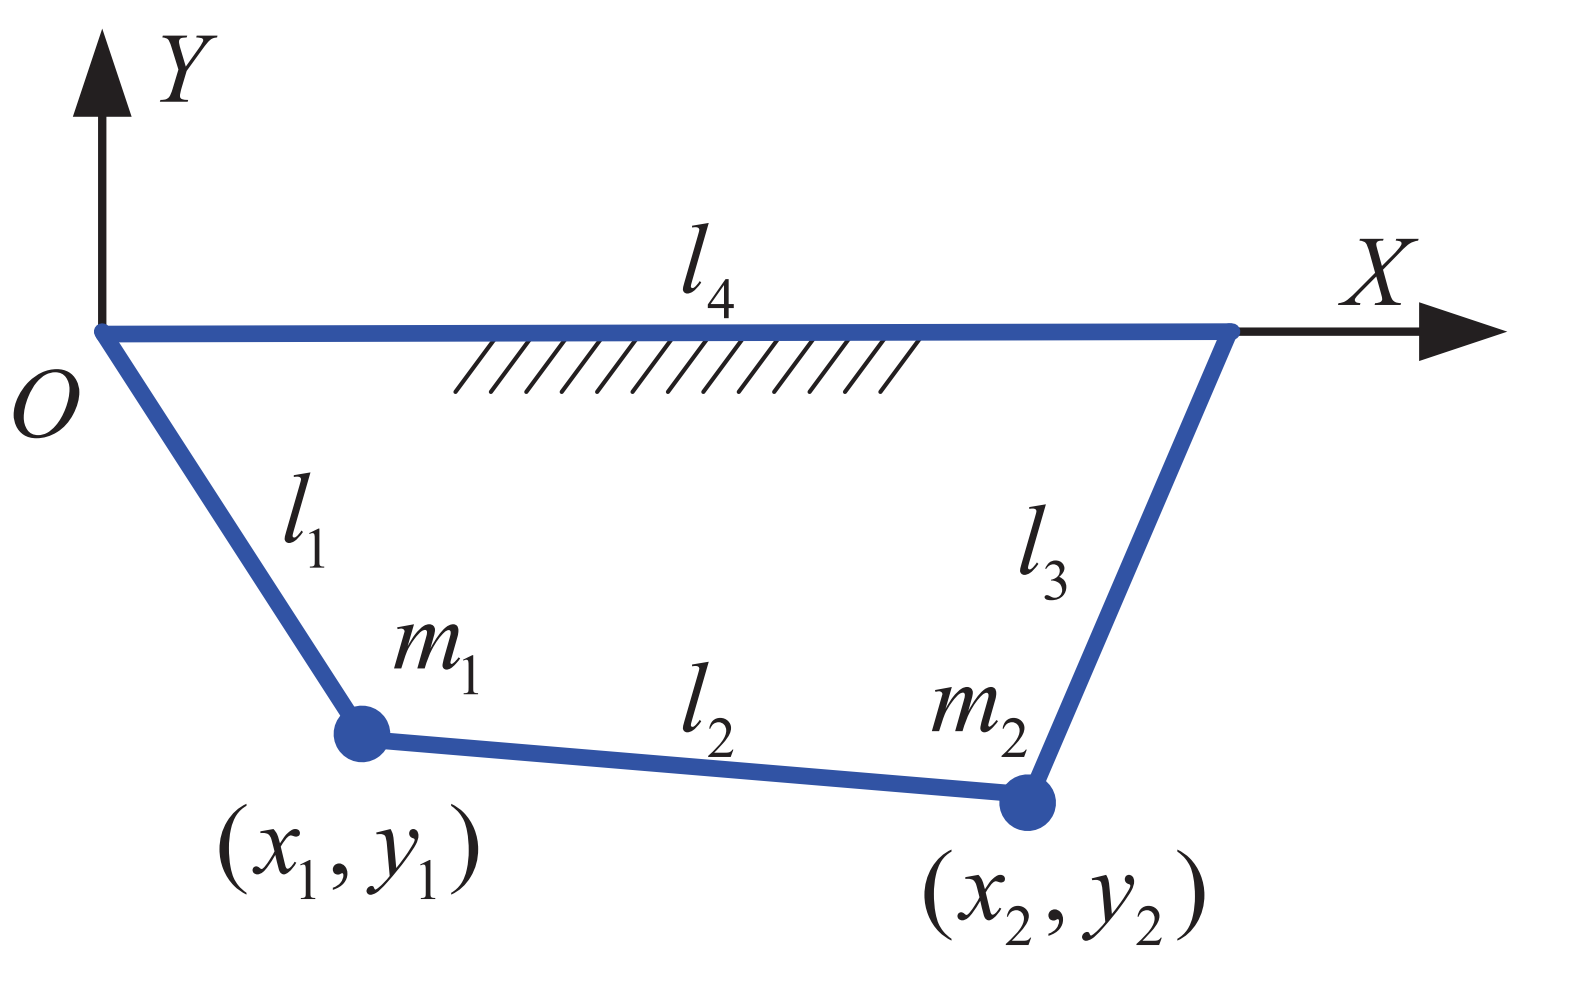
\includegraphics[width=0.6\textwidth]{Figure/有限维广义变分原理_习题.png}
\end{figure}

上图所示为一平面四连杆机构。$OXY$ 为固定参考坐标系；四根杆的长度分别记为 $l_1$、$l_2$、$l_3$ 和 $l_4$；杆 4 固定且与 $X$ 轴共线；不计四根杆的质量，两质点的质量分别记为 $m_1$ 和 $m_2$；重力加速度与 $Y$ 轴同向，沿 $Y$ 轴正向的投影记为 $g$。列写四连杆机构处于重力势能极小值点时两质点坐标 $(x_1, y_1)$ 和 $(x_2, y_2)$ 满足的等式方程。
\end{example}
\begin{solution}
    取两质点的坐标列阵为自变量，即 $\bm{x} = \begin{bmatrix} x_1 & y_1 & x_2 & y_2 \end{bmatrix}^{\mathrm{T}} \in \mathbb{R}^4$。

    第一步：列写约束方程。由连杆长度不变的几何关系可得 $m = 3$ 个约束方程
    \begin{equation*}
        \bm{c}(\bm{x}) = \begin{bmatrix}
            c_1(\bm{x}) \\ c_2(\bm{x}) \\ c_3(\bm{x})
        \end{bmatrix} =
        \begin{bmatrix}
            x_1^2 + y_1^2 - l_1^2 \\
            (x_2 - l_4)^2 + y_2^2 - l_3^2 \\
            (x_2 - x_1)^2 + (y_2 - y_1)^2 - l_2^2
        \end{bmatrix} = \bm{0}.
    \end{equation*}

    第二步：写出目标函数。由于重力加速度沿 $Y$ 轴正向，两质点所受重力分别为 $m_1 g$ 和 $m_2 g$（沿 $Y$ 轴正向），故系统的重力势能为
    \begin{equation*}
        f(\bm{x}) = -g \left( m_1 y_1 + m_2 y_2 \right).
    \end{equation*}

    第三步：计算目标函数的梯度与约束方程的雅可比矩阵
    \begin{equation*}
        \bm{f}_x(\bm{x}) = \frac{\partial f}{\partial \bm{x}} =
        \begin{bmatrix} 0 & -m_1 g & 0 & -m_2 g \end{bmatrix},
    \end{equation*}
    \begin{equation*}
        \bm{c}_x(\bm{x}) = \frac{\partial \bm{c}}{\partial \bm{x}} =
        \begin{bmatrix}
            2x_1 & 2y_1 & 0 & 0 \\
            0 & 0 & 2(x_2 - l_4) & 2y_2 \\
            -2(x_2 - x_1) & -2(y_2 - y_1) & 2(x_2 - x_1) & 2(y_2 - y_1)
        \end{bmatrix}.
    \end{equation*}

    第四步：代入条件极值的必要条件~(\ref{eq:lagrange_cond})，即存在拉格朗日乘子 $\bm{\lambda} = \begin{bmatrix} \lambda_1 & \lambda_2 & \lambda_3 \end{bmatrix}^{\mathrm{T}} \in \mathbb{R}^3$ 使得 $\bm{f}_x^{\mathrm{T}} + \bm{c}_x^{\mathrm{T}}\,\bm{\lambda} = \bm{0}$。将第三步的结果代入并整理，可得如下四个方程
    \begin{equation*}
        \left\{
        \begin{aligned}
            &2x_1 \lambda_1 - 2(x_2 - x_1)\lambda_3 = 0, \\
            &- m_1 g + 2y_1 \lambda_1 - 2(y_2 - y_1)\lambda_3 = 0, \\
            &2(x_2 - l_4)\lambda_2 + 2(x_2 - x_1)\lambda_3 = 0, \\
            &- m_2 g + 2y_2 \lambda_2 + 2(y_2 - y_1)\lambda_3 = 0.
        \end{aligned}
        \right.
    \end{equation*}

    综上，四连杆机构处于重力势能极小值点时，两质点坐标 $(x_1, y_1)$ 和 $(x_2, y_2)$ 与拉格朗日乘子 $\bm{\lambda}$ 共同满足如下 $4 + 3 = 7$ 个等式方程
    \begin{equation}\label{eq:fourbar_cond}
        \left\{
        \begin{aligned}
            &x_1^2 + y_1^2 = l_1^2, \\
            &(x_2 - l_4)^2 + y_2^2 = l_3^2, \\
            &(x_2 - x_1)^2 + (y_2 - y_1)^2 = l_2^2, \\
            &x_1 \lambda_1 - (x_2 - x_1)\lambda_3 = 0, \\
            &y_1 \lambda_1 - (y_2 - y_1)\lambda_3 = \tfrac{1}{2} m_1 g, \\
            &(x_2 - l_4)\lambda_2 + (x_2 - x_1)\lambda_3 = 0, \\
            &y_2 \lambda_2 + (y_2 - y_1)\lambda_3 = \tfrac{1}{2} m_2 g,
        \end{aligned}
        \right.
    \end{equation}
    其中最后四个方程两端已约去公因子 $2$。

    从力学角度看，拉格朗日乘子 $\bm{\lambda}$ 对应三根活动杆的内力（两力杆的拉压轴力），上述后四个方程正是两质点在重力与杆内力作用下的静力平衡条件沿坐标方向的投影。
\end{solution}
